% --- UNIVERSAL PREAMBLE BLOCK ---
\documentclass[12pt, a4paper]{article}

% Margens baseadas no padrão SBC: Sup 3.5cm, Inf 2.5cm, Esq 3.0cm, Dir 3.0cm
\usepackage[a4paper, top=3.5cm, bottom=2.5cm, left=3.0cm, right=3.0cm]{geometry}


\usepackage[portuguese, bidi=basic, provide=*]{babel}

\babelprovide[import, onchar=ids fonts]{portuguese}
\babelprovide[import, onchar=ids fonts]{english}

\usepackage{enumitem}
\setlist[itemize]{label=-}
% --------------------------------

% Pacotes para formatação matemática e citações (Originais do usuário)
\usepackage{amsmath}
\usepackage{amssymb}
\usepackage{amsfonts}
\usepackage[alf]{abntex2cite}
\usepackage{indentfirst} % Recua o primeiro parágrafo de cada seção
\usepackage{graphicx}    % Para incluir as figuras e graficos
\usepackage{booktabs}    % Para tabelas bonitas
\usepackage{float}       % Para posicionar as imagens (parametro H)

% Ajuste de espaçamento de parágrafo padrão da SBC
\setlength{\parindent}{1.27cm}

\begin{document}

% --- CABEÇALHO DO ARTIGO (Estilo SBC) ---
\begin{center}
    {\Large \bfseries Análise Numérica de Circuitos RLC Série: Modelagem da Descarga de Capacitores em Sensores IoT\par}
    \vspace{0.8cm}
    
    {\normalsize     
    \textbf{Antonio Marcos Patrício Castro}\\
    \textbf{Felipe Carneiro de Albuquerque Sarmanho} \\
    \textbf{Pedro Kaic Ribeiro Veloso}
    \par}
    \vspace{0.4cm}
    
    {\normalsize Centro de Ciências Exatas e Tecnologia (CCET) \\
    Universidade Federal do Maranhão (UFMA)\par}
    \vspace{0.2cm}
    
    {\normalsize \textbf{Docente:} Prof. Me. Lucas Reis Abreu\par}
\end{center}

\vspace{0.2cm}

% --- ABSTRACT E RESUMO ---
\begin{quote}
    \noindent\small
    \textbf{Abstract.} \textit{This work presents a numerical study on the solution of Ordinary Differential Equations (ODEs) applied to real-world problems, specifically focusing on IoT signal processing. We analyze the discharge of a capacitor powering a small Internet of Things (IoT) sensor when the main power is cut, modeled by a RLC circuit. Numerical methods are employed to solve the differential equation governing the electric charge over time.}
    
    \vspace{0.3cm} % Espaço entre abstract e resumo
    
    \noindent
    \textbf{Resumo.} \textit{Este trabalho apresenta um estudo numérico sobre a solução de Equações Diferenciais Ordinárias (EDOs) aplicadas a problemas reais, com foco em processamento de sinais IoT. Analisa-se a descarga de um capacitor alimentando um pequeno sensor de Internet das Coisas (IoT) em caso de corte de energia principal, modelado através de um circuito RLC. Métodos numéricos são empregados para resolver a equação diferencial que rege a carga elétrica no tempo.}
\end{quote}

\vspace{0.1cm}

% --- CORPO DO TEXTO ---

A confiabilidade de dispositivos de Internet das Coisas (IoT) depende de sua resiliência a falhas elétricas. Para garantir rotinas de emergência, sensores utilizam fontes como supercapacitores, cuja descarga transiente é modelada por um circuito RLC série e regida por uma Equação Diferencial Ordinária (EDO) de segunda ordem. Evitar oscilações numéricas (ringing) neste regime é essencial para o projeto.

O objetivo central deste estudo é conduzir uma análise comparativa de técnicas matemáticas de solução (Transformada de Laplace, Método de Euler e Runge-Kutta de Quarta Ordem), validando o melhor método para simular a autonomia energética de dispositivos IoT.

\section{Fundamentação Teórica}

\subsection{Transformada de Laplace}

Aplicando a Lei das Malhas de Kirchhoff ao laço sem fonte, a soma das tensões totaliza zero, gerando a equação da carga $q(t)$ \cite{kafle2025, shaikh2022}:
\begin{equation}
    L \frac{d^2q(t)}{dt^2} + R \frac{dq(t)}{dt} + \frac{1}{C} q(t) = 0
\end{equation}

Para a solução analítica ideal, emprega-se a Transformada de Laplace \cite{igwe2025}. Considerando as condições iniciais $q(0) = C V_0$ e $q'(0) = 0$, obtém-se o polinômio característico do sistema:
\begin{equation}
    s^2 + \frac{R}{L} s + \frac{1}{LC} = 0
\end{equation}

Diante da complexidade de modelos reais que impedem soluções analíticas fechadas, algoritmos numéricos como Euler e Runge-Kutta permitem a integração passo a passo da EDO, adaptando-se às variações do sistema \cite{modelagem2026, igwe2025}.

\subsection{Método de Euler}
A aplicação de técnicas numéricas exige a redução da EDO para o espaço de estados, criando duas EDOs de primeira ordem com $x_1(t) = q(t)$ e $x_2(t) = i(t)$ \cite{aselebe2026}:
\begin{equation}
    \begin{bmatrix} x_1' \\ x_2' \end{bmatrix} = \begin{bmatrix} x_2 \\ -\frac{1}{LC}x_1 - \frac{R}{L}x_2 \end{bmatrix}
\end{equation}
O avanço temporal discreto via Euler aproxima a solução iterativamente. Contudo, esse método é condicionalmente estável e sensível à rigidez das oscilações, exigindo passos finos para não divergir.

\section{Runge-Kutta}

Para contornar a deficiência de sobreposições da solução real de Euler, a engenharia recorre à família de métodos de Runge-Kutta. Esses algoritmos consideram a curvatura da função amostrando a derivada em múltiplos pontos por intervalo \cite{firgelli2026rk, stackexchange2015}. O Runge-Kutta de Quarta Ordem (RK4) é o mais adotado \cite{shaikh2022}. Ele projeta o estado avaliando quatro inclinações ($k_1, k_2, k_3, k_4$) intermediárias \cite{razak2025}:
\begin{align}
    k_1 &= \mathbf{f}(t_n, \mathbf{x}_n) \\
    k_2 &= \mathbf{f}(t_n + \frac{h}{2}, \mathbf{x}_n + \frac{h}{2}k_1) \\
    k_3 &= \mathbf{f}(t_n + \frac{h}{2}, \mathbf{x}_n + \frac{h}{2}k_2) \\
    k_4 &= \mathbf{f}(t_n + h, \mathbf{x}_n + h k_3)
\end{align}
\begin{equation}
    \mathbf{x}_{n+1} = \mathbf{x}_n + \frac{h}{6} (k_1 + 2k_2 + 2k_3 + k_4)
\end{equation}

O poder computacional do RK4 reside na tolerância a erros. O erro global acumulado escala na ordem de $\mathcal{O}(h^4)$ \cite{modelagem2026}. Isso propicia uma convergência extraordinariamente mais rápida se comparada à do Método de Euler \cite{firgelli2026rk}.

\section{Metodologia Computacional}

A implementação inicializa o sensor no corte de energia com $i(0) = 0$ e tensão de operação $V_0 = 3{,}3\,\text{V}$ \cite{igwe2025}. Os parâmetros físicos do circuito subamortecido foram fixados em $R = 2\,\Omega$, $L = 10\,\text{mH}$ e $C = 100\,\mu\text{F}$ \cite{shaikh2022}. O simulador resolve iterativamente o Método de Euler e RK4 a cada passo $h$, convertendo as cargas na tensão disponível $V_C(t)$ \cite{aselebe2026}. O código foi desenvolvido em \textit{Python}, utilizando \textit{NumPy} para integração vetorial e \textit{Matplotlib} para gráficos analíticos \cite{igwe2025}.


\section{Resultados e Discussões}

A simulação abrangeu $t_{\text{final}} = 15\,\text{ms}$, empregando $n = 60$ passos ($h = 0{,}25\,\text{ms}$). A resistência $R = 2\,\Omega$ submete o circuito a um regime dinâmico subamortecido crítico, provocando oscilações severas que desafiam aproximações lineares.

\subsection{Dinâmica da Tensão}
A Figura~\ref{fig:comparacao} sobrepõe as estimativas numéricas à solução exata de Laplace. Observa-se que o RK4 se funde perfeitamente à solução analítica. Já o Método de Euler demonstra dificuldades severas nas porções curvas, resultando em desvios consideráveis da tensão.

\begin{figure}[H]
    \centering
    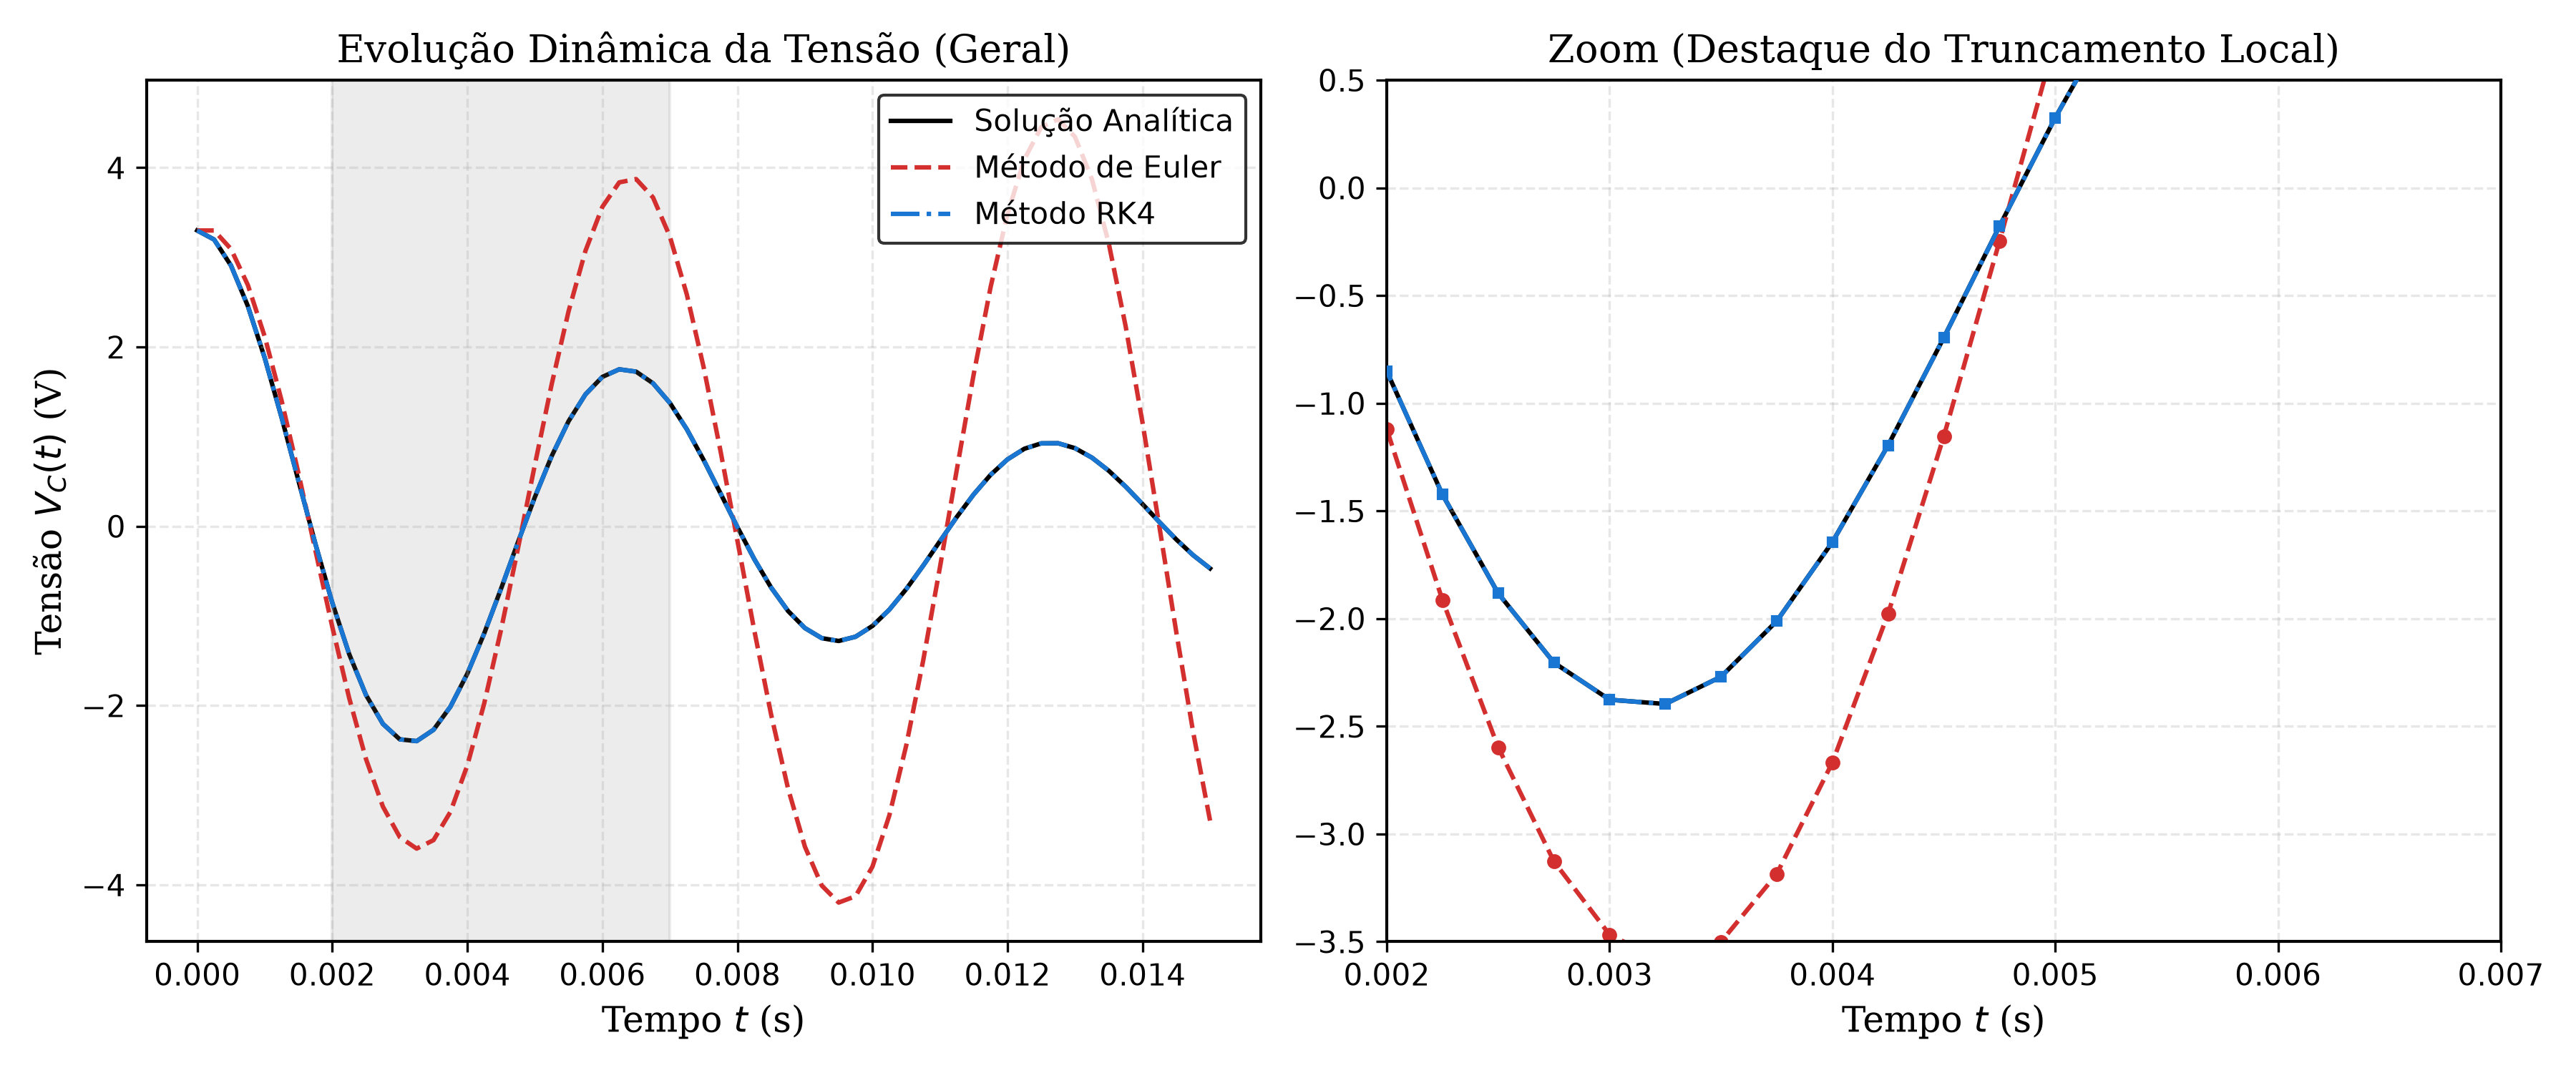
\includegraphics[width=0.75\textwidth]{comparacao_metodos.png}
    \caption{Curvas de tensão derivadas pela solução exata, Euler e RK4 ($n = 60$).}
    \label{fig:comparacao}
\end{figure}

A Tabela~\ref{tab:resultados} quantifica os erros absolutos. O RK4 preserva a fidelidade (erro de $10^{-4}$ V), contra falhas grosseiras na ordem de Volts ($10^{0}$ V) no Euler.

\begin{table}[H]
    \centering
    \caption{Erros absolutos extraídos nos principais instantes ($n = 60$).}
    \label{tab:resultados}
    \begin{tabular}{ccccc}
        \toprule
        $t$ (ms) & Analítico (V) & Euler (V) & RK4 (V) & Erro Euler (V) \\
        \midrule
        0,00 & 3,300000 & 3,300000 & 3,300000 & 0,000000 \\
        3,75 & $-$2,011858 & $-$3,185733 & $-$2,012058 & 1,17$\times 10^{0}$ \\
        7,50 & 0,739721 & 1,774930 & 0,740103 & 1,03$\times 10^{0}$ \\
        11,25 & 0,105210 & 0,634171 & 0,104838 & 5,28$\times 10^{-1}$ \\
        15,00 & $-$0,469621 & $-$3,283289 & $-$0,469416 & 2,81$\times 10^{0}$ \\
        \bottomrule
    \end{tabular}
\end{table}

\subsection{Discussão de Erros e Convergência Algorítmica}

A discrepância tabelada levou ao estudo do erro temporal (Figura~\ref{fig:erro}). O RK4 é superior porque avalia quatro pontos por passo e pondera a curvatura, enquanto Euler, de primeira ordem, usa apenas uma reta inicial, tornando-se cego a variações.

Esse limite causa uma explosão do erro numérico em passos largos. A Figura~\ref{fig:erro} evidencia o desvio do Euler atingindo $3{,}61$ V (valor que supera a própria fonte de $3{,}3$ V), enquanto o RK4 retém precisão microscópica ($4{,}01 \times 10^{-4}$ V), validando sua exatidão absoluta.

\begin{figure}[H]
    \centering
    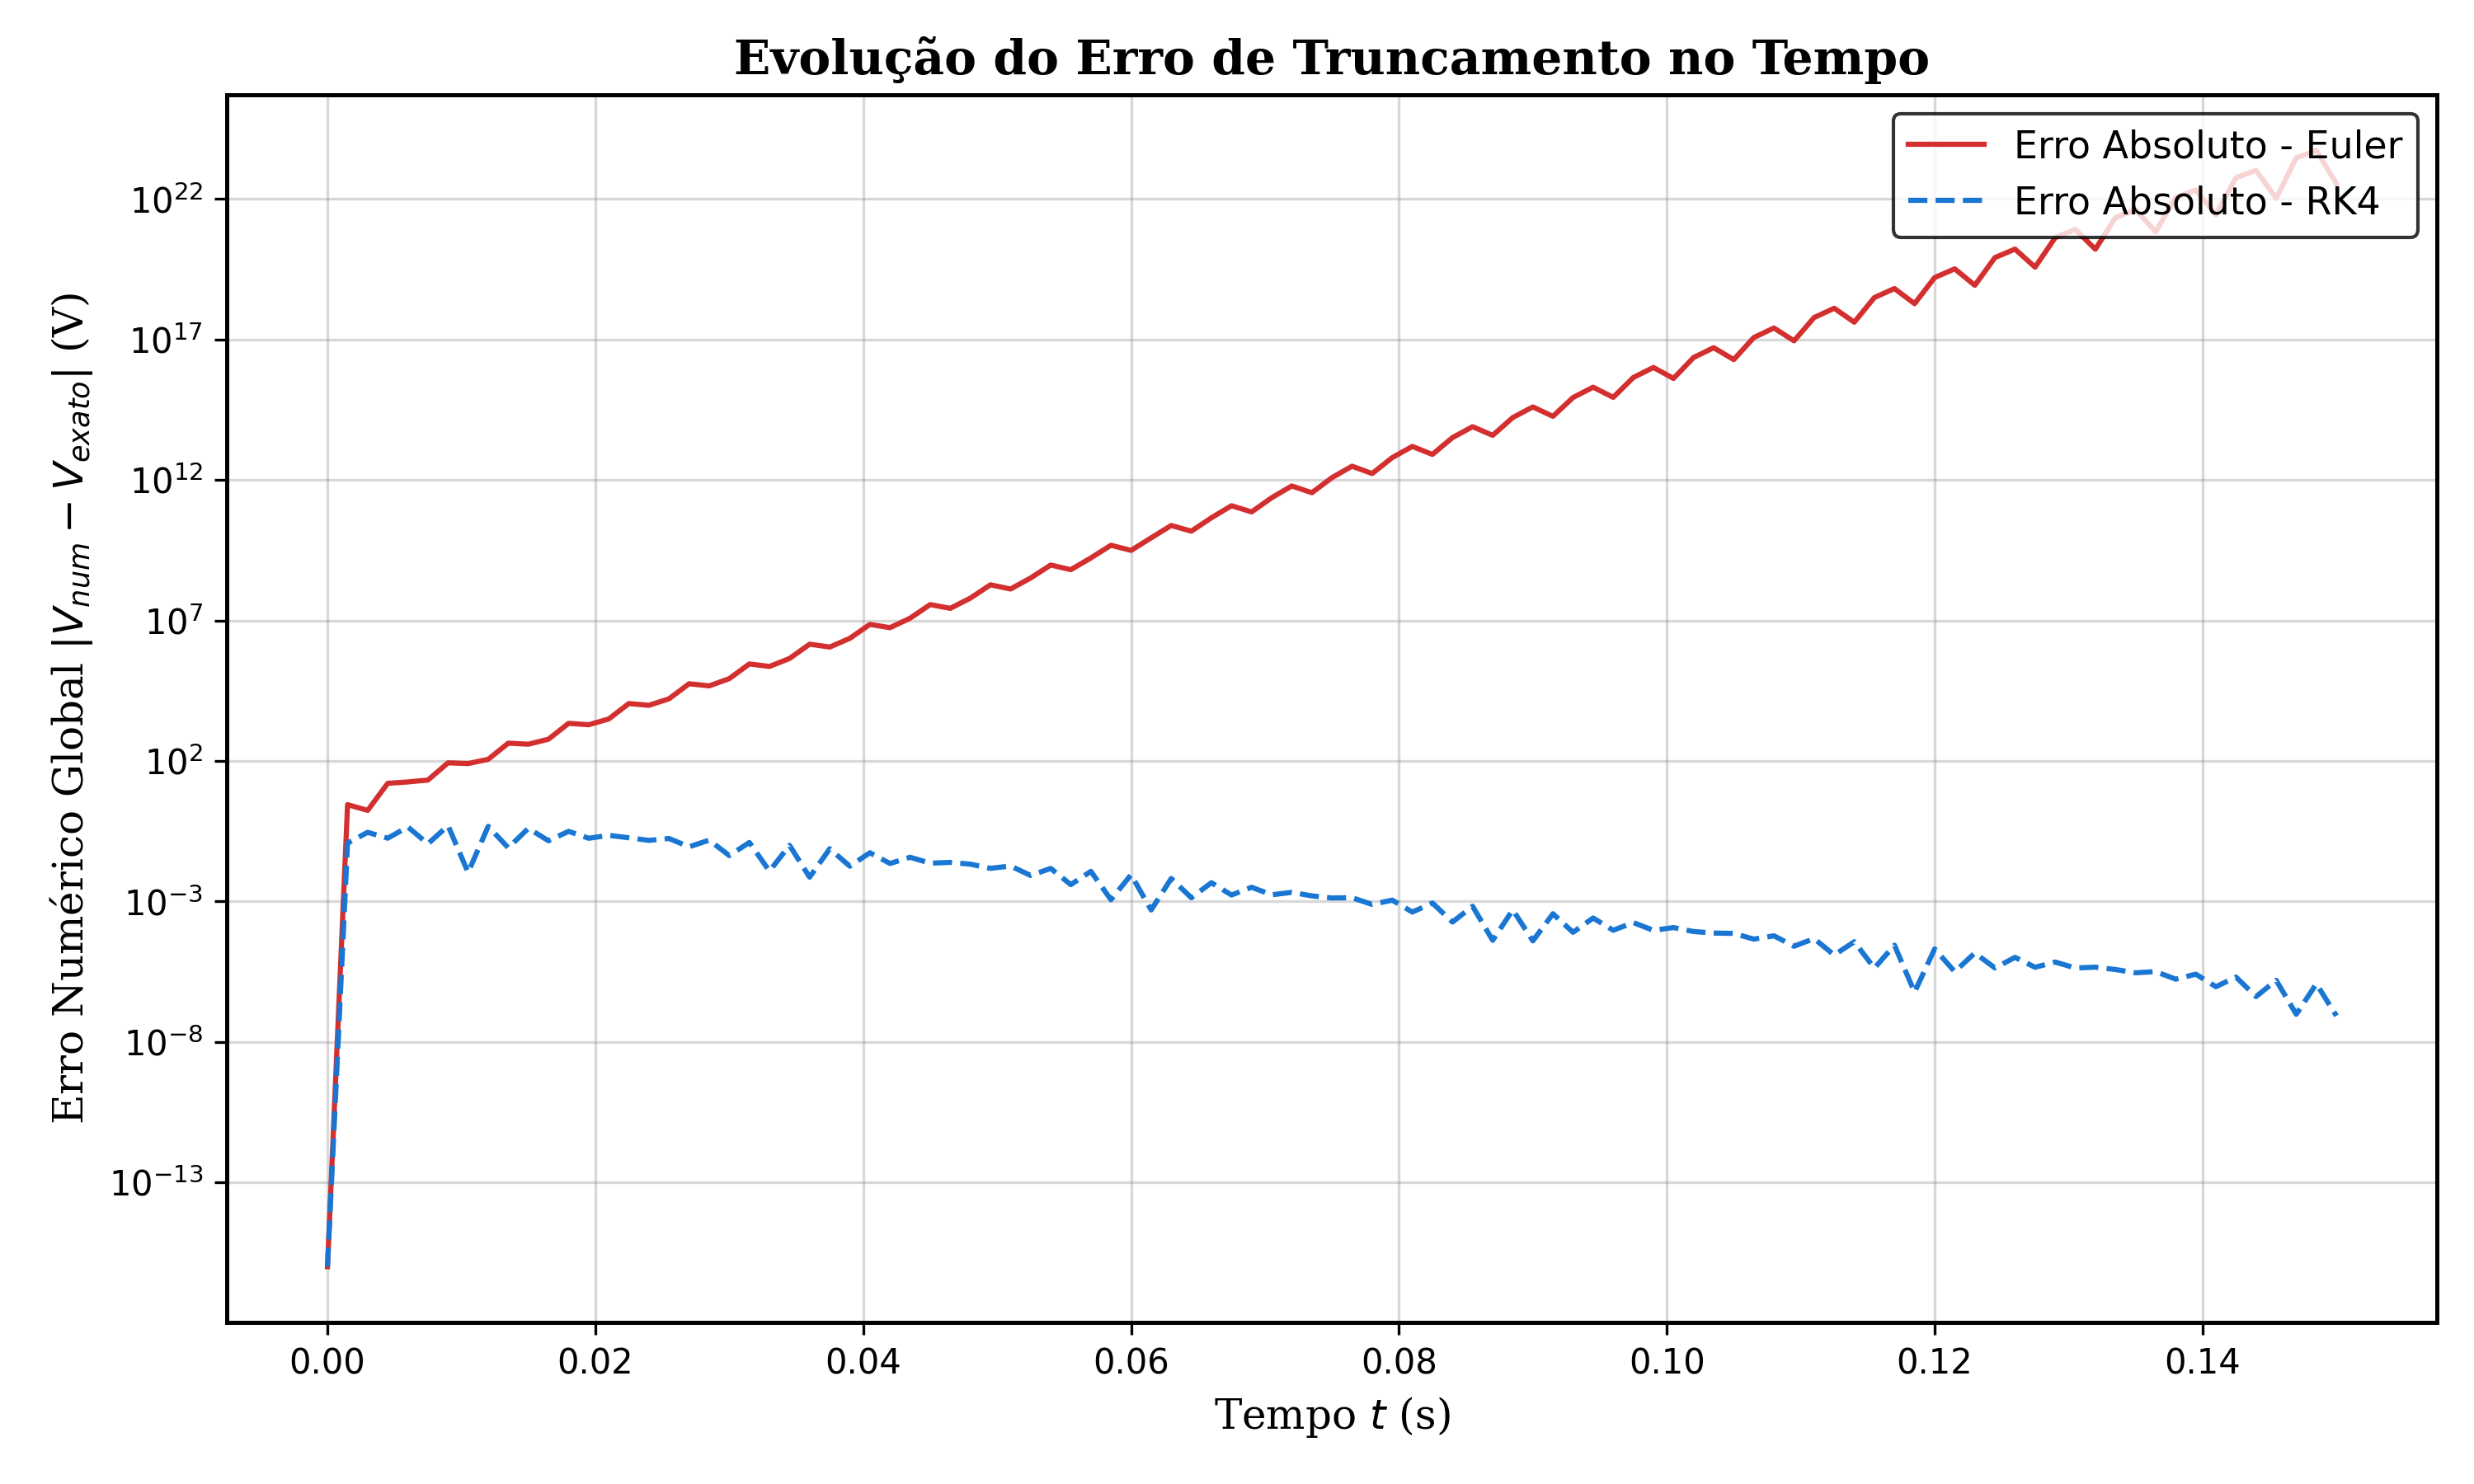
\includegraphics[width=0.75\textwidth]{erro_absoluto.png}
    \caption{Erro absoluto de tensão no tempo (Euler e RK4).}
    \label{fig:erro}
\end{figure}

Por fim, o teste de convergência (Figura~\ref{fig:convergencia}) prova os teoremas. A reta de Euler evidencia queda linear de resíduos $\mathcal{O}(h)$, e o RK4 apresenta queda acentuada $\mathcal{O}(h^4)$, sem onerar exaustivamente o processador.

\begin{figure}[H]
    \centering
    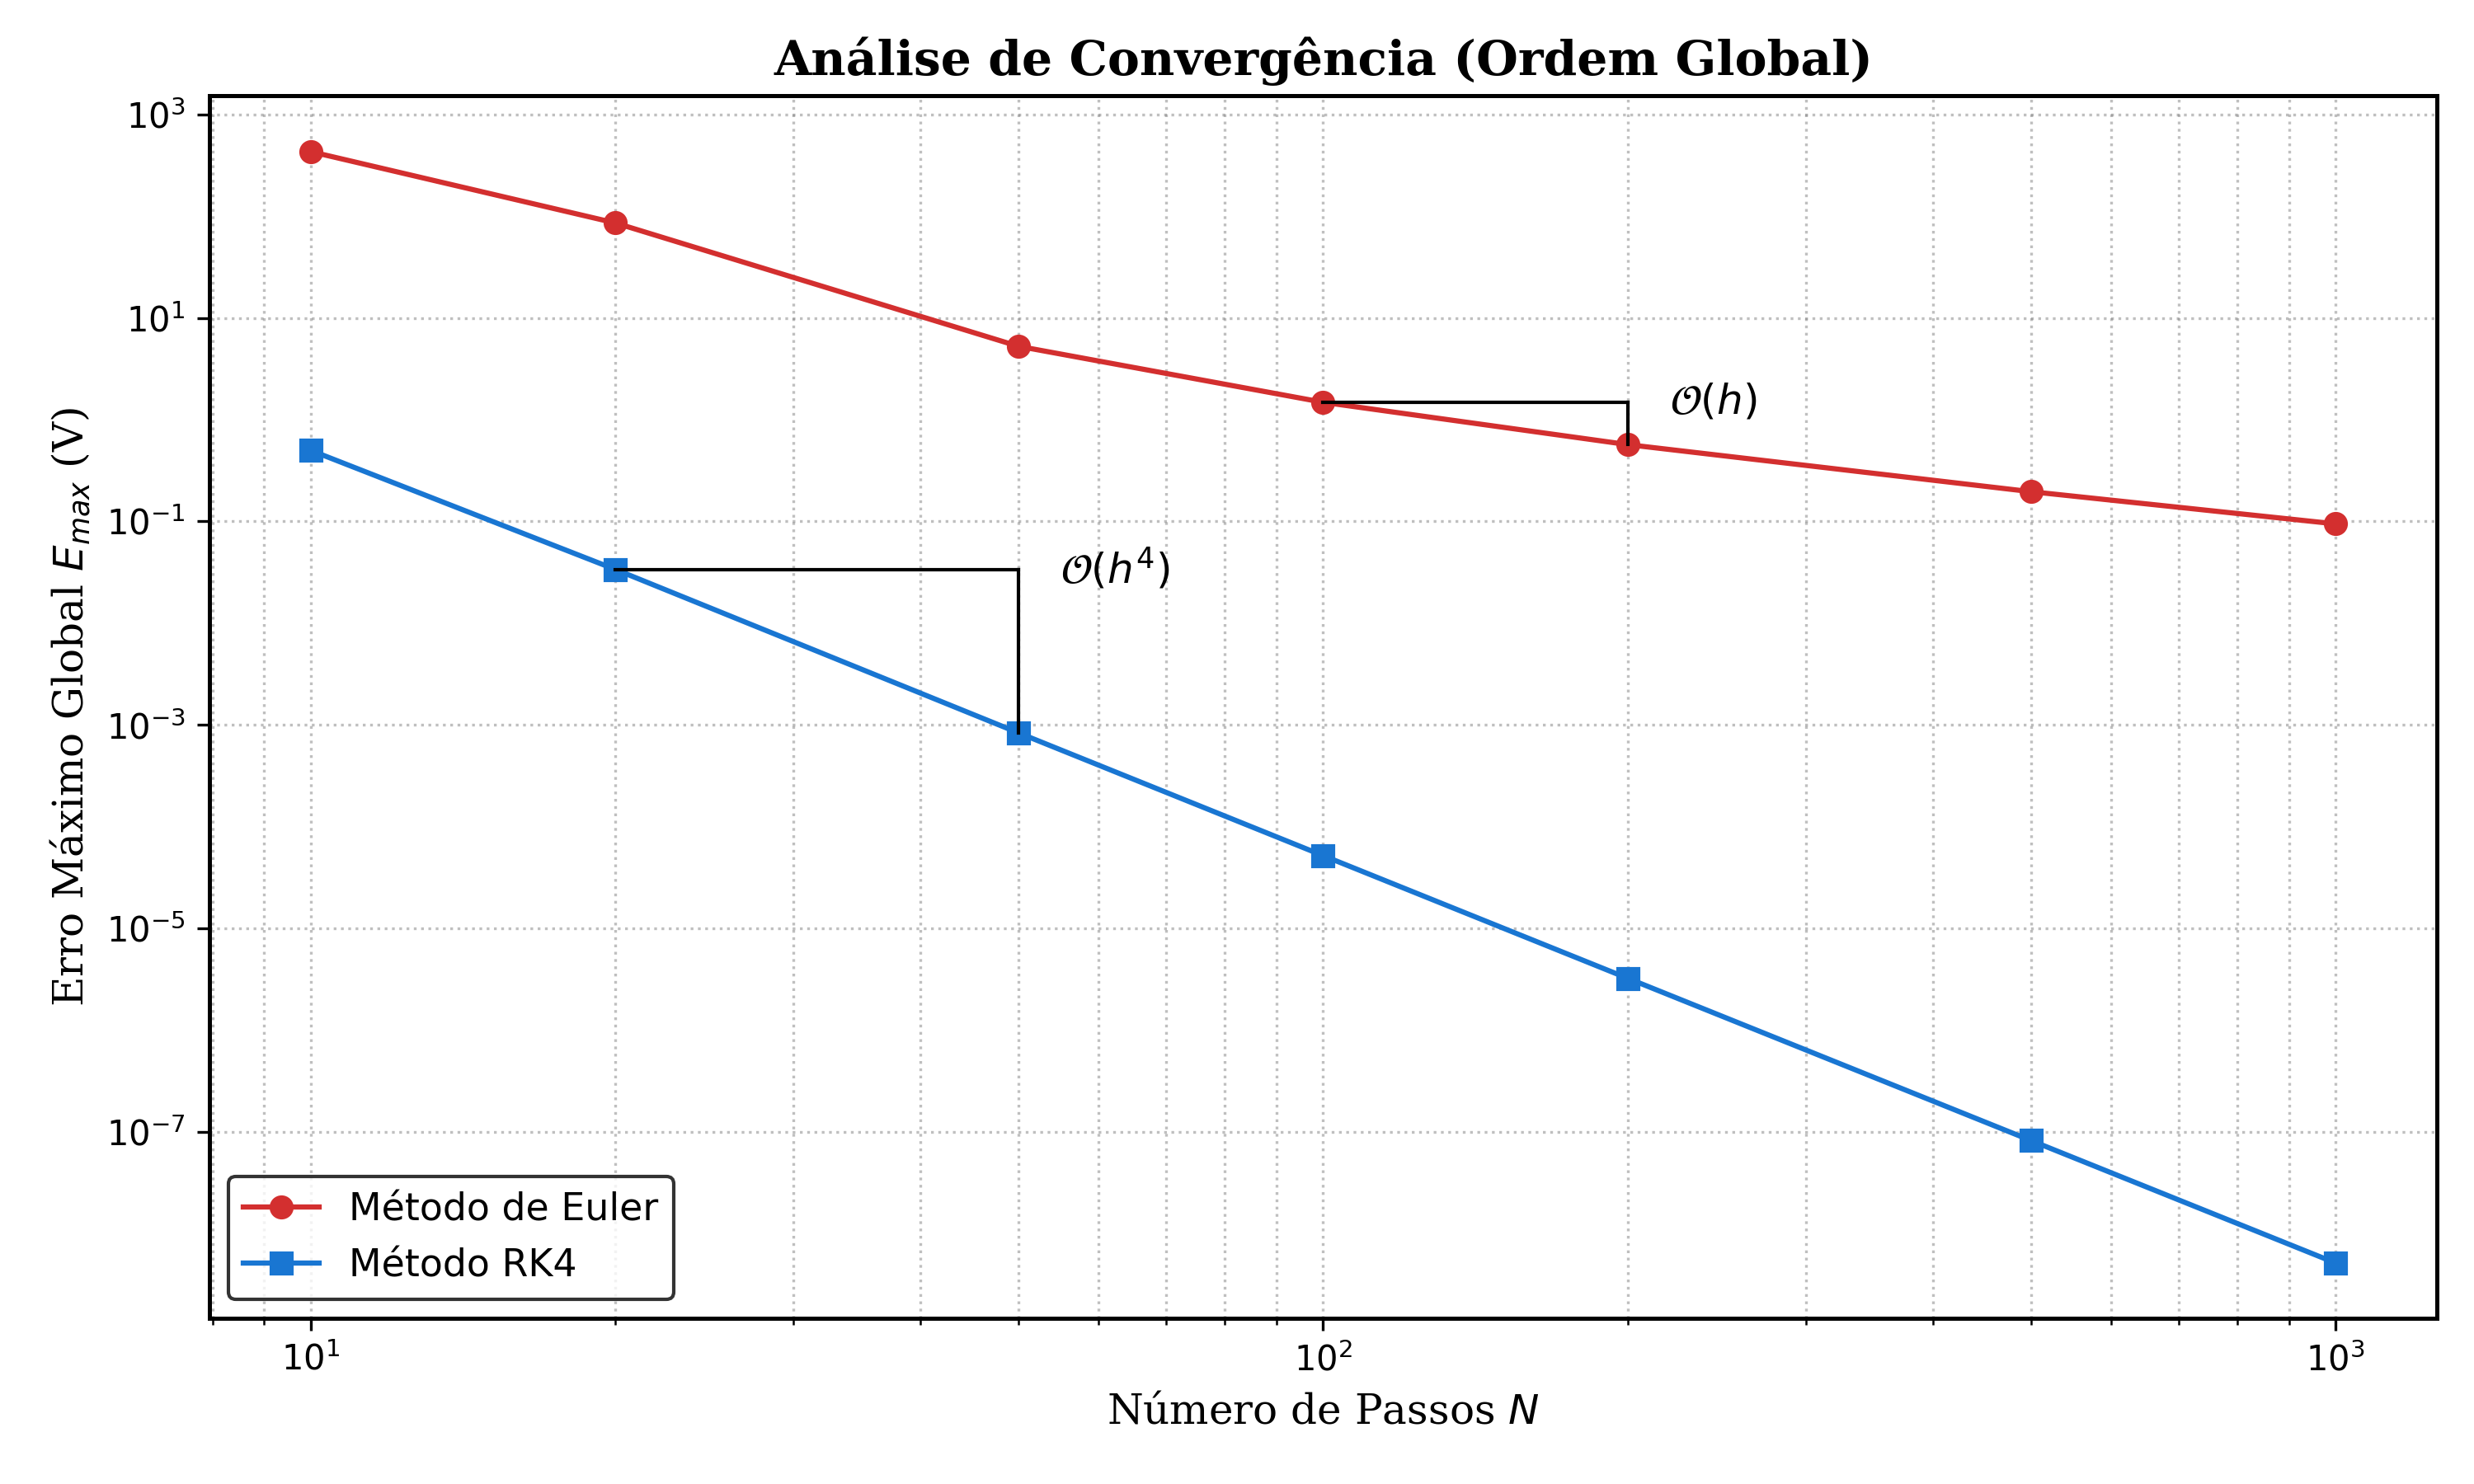
\includegraphics[width=0.75\textwidth]{convergencia.png}
    \caption{Convergência correlacionando Erro Máximo com número de passos ($n$).}
    \label{fig:convergencia}
\end{figure}


\section{Considerações Finais}

A utilização do Cálculo Numérico na modelagem de sistemas embarcados e dispositivos IoT prova-se de extrema importância. A capacidade de prever a curva de descarga de capacitores utilizando sistemas de EDOs permite o dimensionamento correto de componentes, garantindo a viabilidade e a segurança do processamento de sinais mesmo em condições de falha de energia.

\clearpage
% --- REFERÊNCIAS BIBLIOGRÁFICAS ---
% Usando o ambiente thebibliography para manter o documento num arquivo único.
% Chamada do arquivo de referências (referencias.bib)
\bibliography{referencias}

\end{document}